\documentclass[a4paper]{article}

\usepackage{pgfplots}

\begin{document}

\begin{tikzpicture}
%\tracingcommands=2\tracingmacros=2
	\begin{axis}[
		clip=false,
		symbolic x coords={A,B},
		xtick={A,B},
		nodes near coords={%
			\begingroup
			\pgfplotspointgetnormalizedcoordinates
			$N = (
				\pgfmathprintnumber{\pgfkeysvalueof{/data point/x}},
				\pgfmathprintnumber{\pgfkeysvalueof{/data point/y}})$
			\endgroup
			\pgfplotspointgetcoordinates
			$A = (
				\pgfkeysvalueof{/data point/x},
				\pgfmathprintnumber{\pgfkeysvalueof{/data point/y}})$
		},%
	]

	\addplot coordinates {(A,1) (B,2)};

	\end{axis}
\end{tikzpicture}

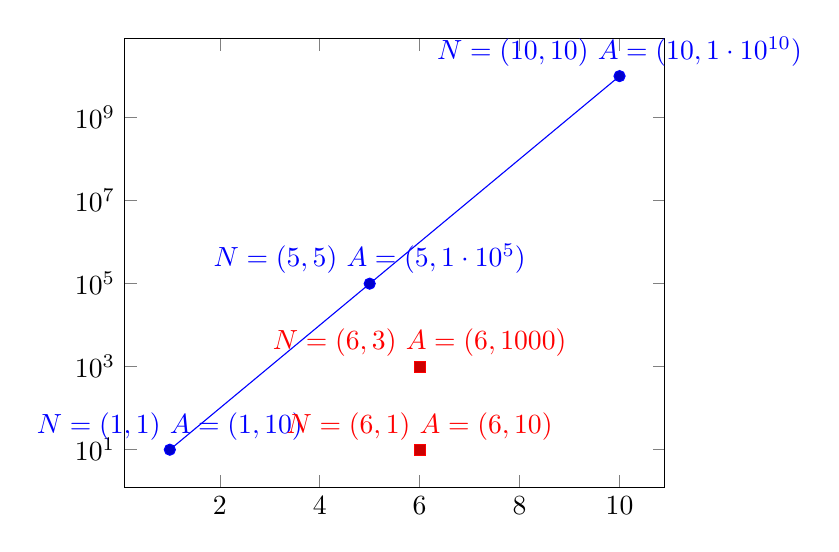
\begin{tikzpicture}
%\tracingcommands=2\tracingmacros=2
	\begin{semilogyaxis}[
		log basis y=10,
		nodes near coords={%
			\begingroup
			\pgfplotspointgetnormalizedcoordinates
			$N = (
				\pgfmathprintnumber{\pgfkeysvalueof{/data point/x}},
				\pgfmathprintnumber{\pgfkeysvalueof{/data point/y}})$
			\endgroup
			\pgfplotspointgetcoordinates
			$A = (
				\pgfmathprintnumber{\pgfkeysvalueof{/data point/x}},
				\pgfmathprintnumber{\pgfkeysvalueof{/data point/y}})$
		},%
		/pgf/number format/1000 sep={},
	]
		
	\addplot+[domain=1e0:1e1,samples at={1,5,10}] {10^x};

	\addplot+[only marks] coordinates {(6,1e1) (6,1e3)};

	\end{semilogyaxis}
\end{tikzpicture}
\end{document}

